\chapter{Metodi Multivariati e i Boosted Decision Tree}

\section{Analisi Multivariata e Problemi di Selezione} \label{AnalisiMulti}
In questa tesi le candidate $D^{*+}$ sono state selezionate utilizzando algoritmi di apprendimento artificiale. L'apprendimento artificiale (in inglese "machine larning") \`e un meccanismo che permette ad una macchina di migliorare le proprie prestazioni nel tempo. \cite{sitoMachineLearning}
\\L'apprendimento artificiale consiste nello sviluppo di algoritmi che possono imparare dai dati e in base ad essi prendere decisioni o fare previsioni. L'apprendimento artificiale può essere di tipo supervisionato o non supervisionato. Nel primo caso per addestrare l'algoritmo si utilizzano degli esempi di cui si fornisce anche la "risposta". In questo modo vi è una sorta di feedback su cui si basa l'addestramento dell'algoritmo. Nel caso non supervisionato, al contrario, vengono forniti solo dei dati e sarà l'algoritmo stesso a decidere indipendentemente come classificarli. 

In particolare, in questa tesi \`e stato utilizzato un metodo di analisi multivariata, cioè un metodo di analisi statistica basato sull'analisi congiunta di più variabili. L'\textit{analisi multivariata}  appartiene al caso dell'apprendimento artificiale supervisionato e combina una serie di variabili discriminatorie di input in un'unica variabile discriminatoria finale, chiamata \textit{classifier output}.
\\In questa tesi si affronta un \textit{problema di selezione}, ovvero si cerca un segnale raro in un insieme composto principalmente da eventi di fondo, quindi il rapporto segnale su fondo \`e molto minore di 1, perciò un'analisi multivariata potrebbe portare a performance migliori nell'identificazione del segnale.
Per l'analisi svolta in questa tesi \`e stato utilizzato il "TMVA" \cite{TMVA} (Tool for MultiVariate Analysis), che \`e uno strumento incluso nel framework ROOT\cite{Root} che implementa diversi metodi di analisi multivariata.

L'analisi effettuata con i metodi di apprendimento artificiale si struttura in due fasi principali:
    \begin{itemize}
        \item Training: in questa fase l'algoritmo viene istruito a separare il segnale dal fondo fornendo un campione di dati di cui è noto quali rappresentino il segnale e quali il fondo. Vengono anche indicate quali sono le variabili discriminatorie che l'algoritmo deve usare per separare i due insiemi;
        \item Applicazione: nella fase di applicazione viene utilizzato quanto appreso dalla macchina nella fase di training per selezionare e dividere il segnale dal fondo.
    \end{itemize}
    
\section{Boosted Decision Tree} \label{BDT}

    \subsection{Alberi decisionali}
    Un \textit{albero decisionale} (decision tree) è una struttura che classifica i dati mediante scelte di tipo binario. Se ne riporta uno schema esemplificativo in figura \ref{fig:BDT}. Ogni scelta è basata su una selezione su una singola variabile. %Ogni scelta è basata su un taglio su una singola variabile.
    Ogni ramo creato viene poi nuovamente diviso in due in base alla selezione su un'altra variabile. I gruppi di dati creati alla fine dell'albero sono chiamati foglie. Le foglie vengono identificate come segnale o fondo in base alla classe cui appartiene la maggior parte degli eventi. 
    
    \begin{figure}[htbp]
        \centering
        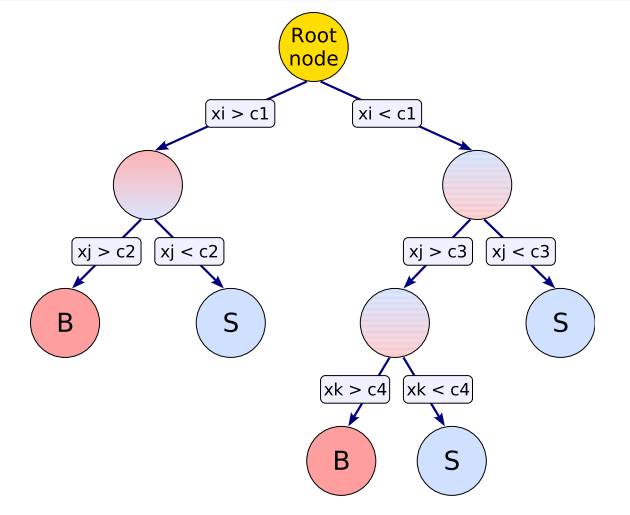
\includegraphics[width=0.5\linewidth]{TMVA/BDT1.PNG}
        \caption{ Esempio di schema di un albero decisionale. Le variabili $xi, \ xj, \ xk$ indicate nello schema sono le variabili discriminatorie, gli elementi dell'albero con la lettera S sono le "foglie" dell'albero, ovvero gli insiemi di dati, selezionati come segnale, mentre gli elementi con la lettera B sono quelli selezionati come fondo.}
        \label{fig:BDT}
    \end{figure}
    
    Un vantaggio degli alberi decisionali è che sono facilmente visualizzabili ed è altrettanto semplice ricondursi al significato fisico delle selezioni operate. Inoltre sono perlopiù insensibili alla presenza di variabili poco discriminanti. Lo svantaggio principale è che sono fortemente sensibili alle fluttuazioni statistiche dei dati utilizzati per il training. Questo problema viene risolto con il "boosting" di cui si parla nella sezione  \ref{Boosting}.
    \\La prima divisione dei dati, chiamata root node, viene scelta individuando la variabile e il relativo valore di selezione che meglio divide i dati tra segnale e fondo. L'indice di separazione utilizzato in questa tesi è quello di Gini \footnote{L'indice di Gini è definito come: $p (1-p)$, dove $p$ è la purezza del segnale, che è il rapporto tra il numero di eventi segnale e il numero di eventi totale}. A questo punto si considera singolarmente ognuno dei due rami e si sceglie la selezione sulla variabile che massimizza l'aumento dell'indice di separazione.
    \\Infine è necessario fare un controllo per l'\textit{overtraining}, ovvero la possibilità che l'albero decisionale sia troppo dipendente dal campione di dati utilizzati nella fase di training e non sia più descrittivo del fenomeno fisico nella sua generalità. Per fare ciò si fa classificare all'algoritmo delBDT in segnale e fondo un campione di dati detto campione di test, di cui si consce a priori se siano segnale o fondo.
 
    \subsection{Boosting} \label{Boosting}
    Per migliorare le performance dell'algoritmo di apprendimento artificiale si pu\`o utilizzare il meccanismo del \textit{boosting}. Questo viene utilizzato nel caso degli alberi decisionali per renderli più stabili rispetto alle fluttuazioni statistiche del set di dati del training e per migliorarne la capacit\`a di discriminare tra segnale e fondo. Per fare ciò l'algoritmo ripete automaticamente il training pi\`u volte utilizzando lo stesso campione di dati e ad ogni ripetizione assegna pesi diversi ai dati classificati erroneamente.
    \\L'algoritmo di boosting utilizzato in questa tesi è l'\textit{Adaptive Boosting} (AdaBoost). In questo caso i dati che sono stati classificati erroneamente nel precedente albero decisionale vengono ripesati con un fattore $\alpha$, che è calcolato come 
        \begin{equation}
            \alpha = \frac{1 - err}{err}
        \end{equation}
    dove $err$ è il rate di eventi classificati erroneamente. 
    \\Si viene a creare una insieme di alberi decisionali da cui si deriva il responso finale. Gli algoritmi di boosting funzionano meglio se si utilizzano alberi piccoli, ovvero con pochi livelli di diramazione.
    
